\section{Aufbau}
\label{sec:Aufbau}

Die vier Probestäbe sind mit einem Peltierelement verbunden, welches die Stäbe bei Betrieb auf einer Seite erhitzt beziehungsweise kühlt. Die Temperaturen werden durch Thermoelemente an den gekennzeichneten Stellen abgegriffen. Über ein Temperatur Array werden die Informationen an einen Xplorer GLX weitergegeben. Mit dem Schalter kann das Peltierelement auf heizen oder kühlen gestellt werden.

\begin{figure}
	\centering
	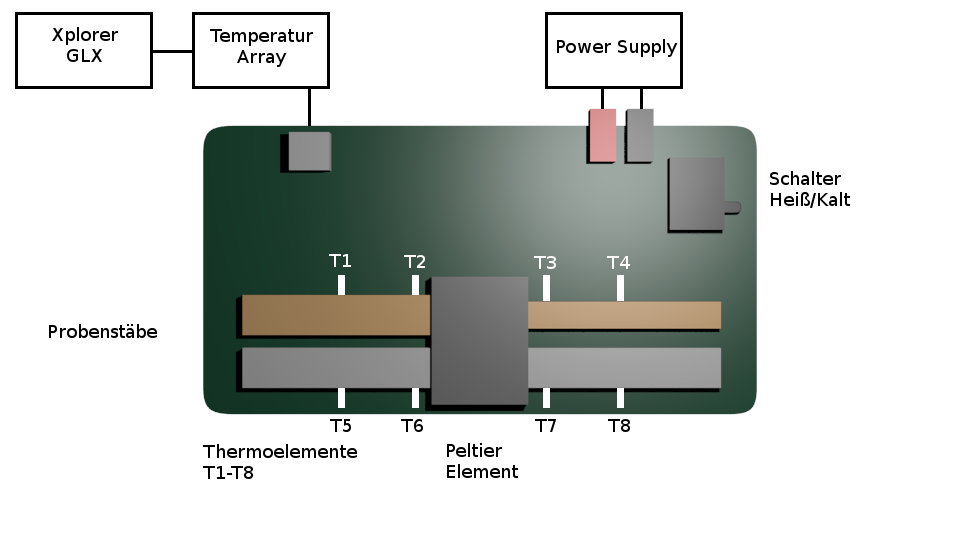
\includegraphics[scale = .45,keepaspectratio]
	{content/images/Aufbau.png}
	\caption{Schema des Versuchaufbaus}
	\label{fig:Aufbau}
\end{figure}